\chapter{Supplementary Results}
\label{CHAPTER:APPENDIX}
\centerline{\rule{149mm}{.02in}}
\vspace{2cm}

\section{Network Results}

This section reports results on the effect of the mean degree on performance of
a system, in an effort to determine the optimal mean degree value for our
system. This value has to balance several key properties. It has to high enough
to give a good connectedness level in the network, to allow for a good expose
to jobs.  It has to be low enough that the middleware handling the messages is
not overloaded by communication costs.  If the mean degree is close to the
network size, the topology becomes more like an all-to-all network, and our
topology experiments have less meaning. Also given we are simulating a
massively parallel process on a single machine, some consideration mush be
given to the simulation run time, which dramatically increased with the mean
degree. These results show a simulation on a grid of size 1024, using the base
ZI trader/sealed bid/random network auction market, across a range of mean
degree values. Each results shows the mean of 10 simulation runs.

A value of 128 was chosen as a compromise between the previously discussed
aspects, particularly to improve the simulation's execution time.

\begin{figure}[h] 
  \centering
  \fbox{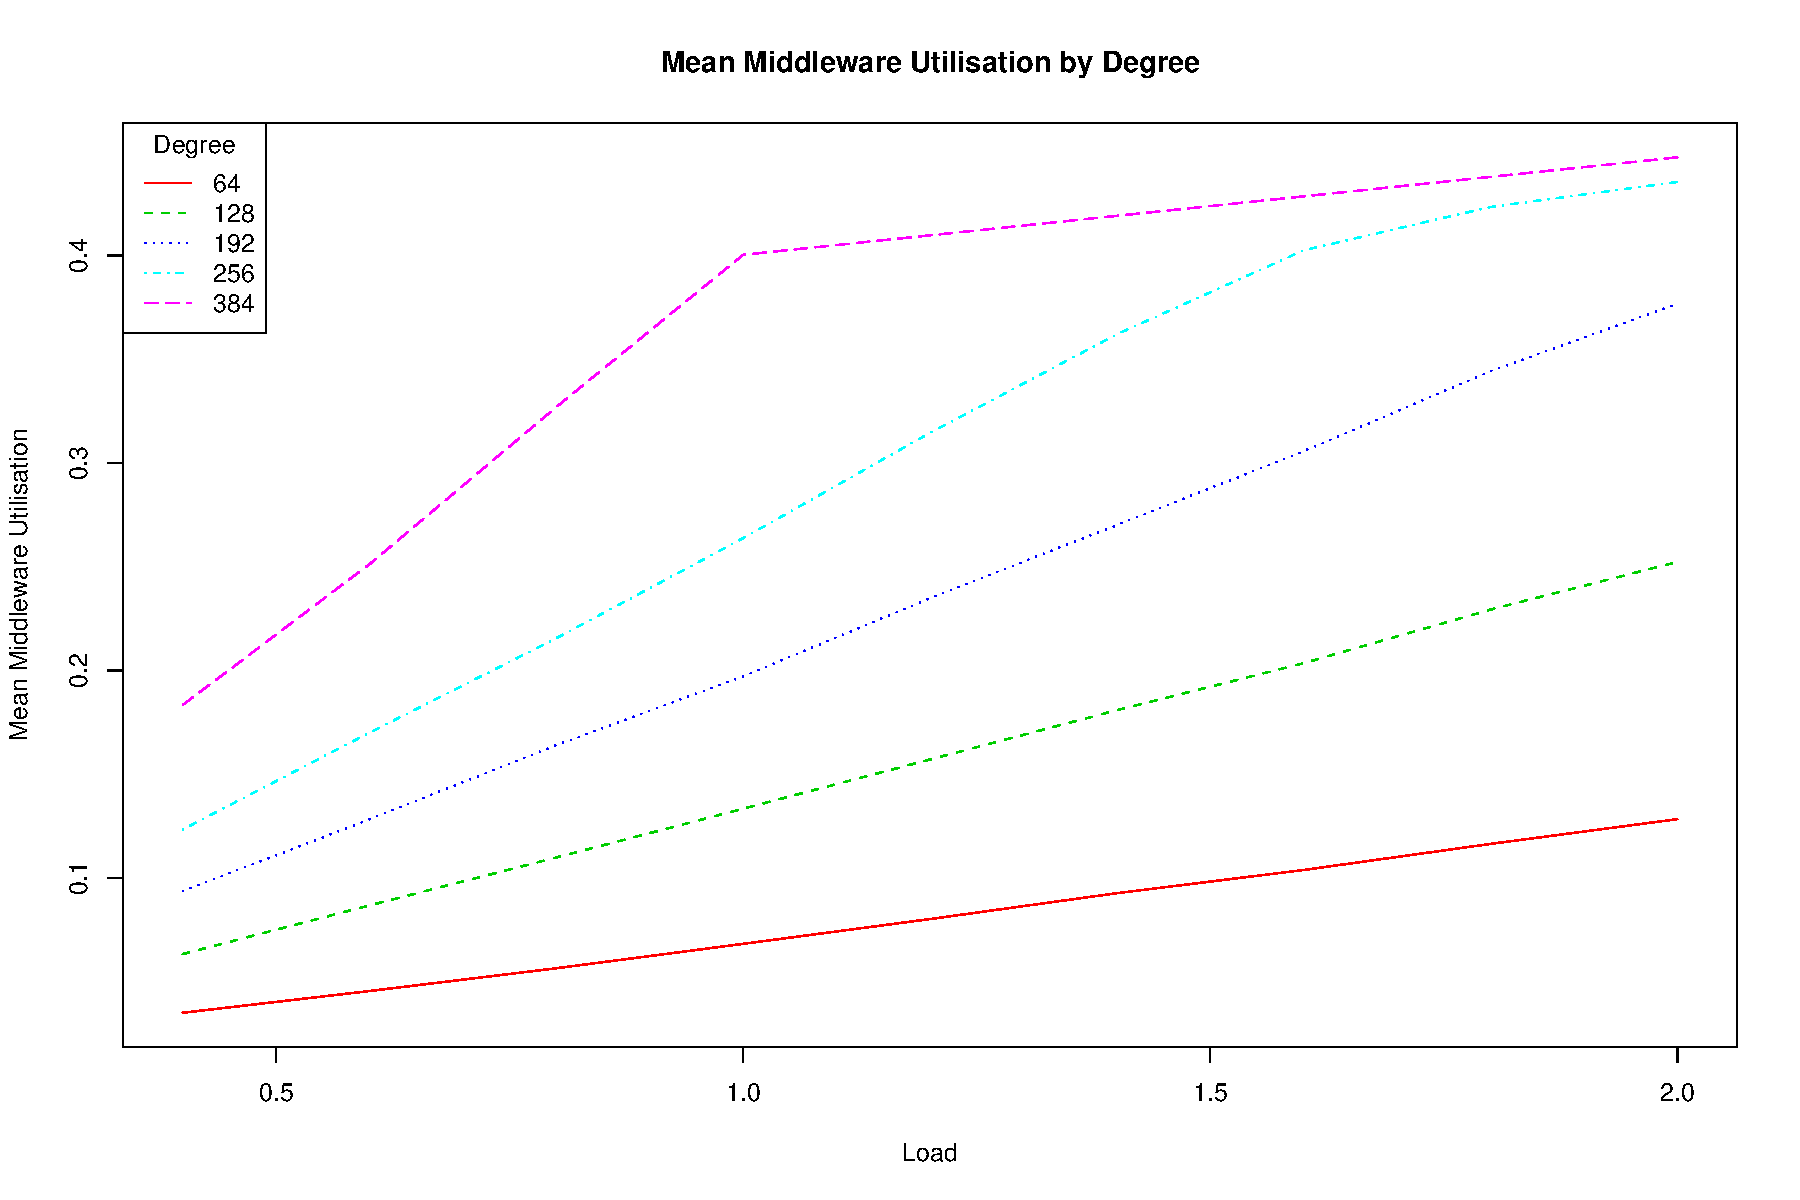
\includegraphics[width=12cm]{appendix/middleware_util_mean}}
  \label{FIG:APX:MUTIL}
  \caption{The mean middleware utilisation for systems with the base system of
  size 1024. Even for high degree values, the load is at sensible levels.}
\end{figure}

\begin{figure}[h] 
  \centering
  \fbox{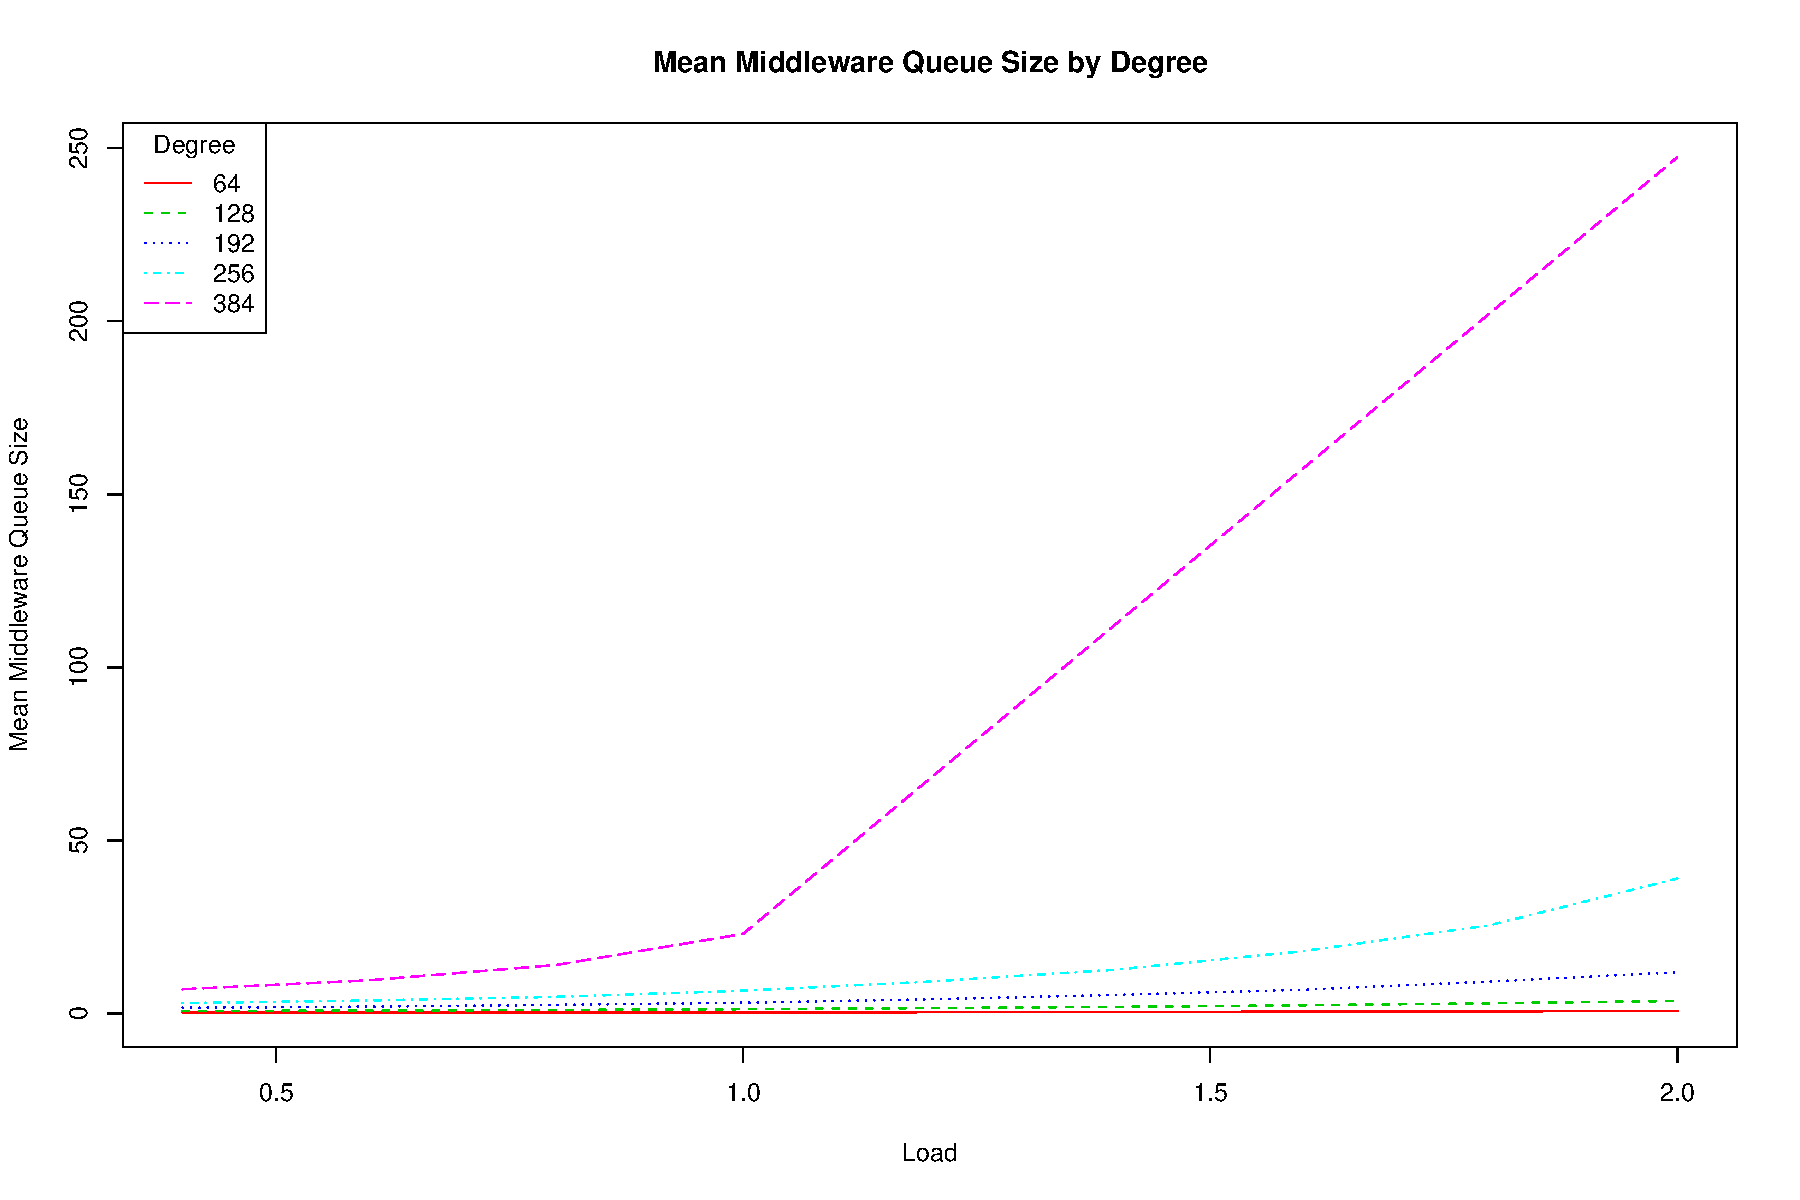
\includegraphics[width=12cm]{appendix/queue_size_mean}}
  \label{FIG:APX:QSIZE}
  \caption{The mean size of the middleware's message queue. This shows the
  degree of concurrent message handling which the middleware has to handle. For
  a degree of 384, you can clearly see the significant increase}
\end{figure}

\begin{figure}[h] 
  \centering
  \fbox{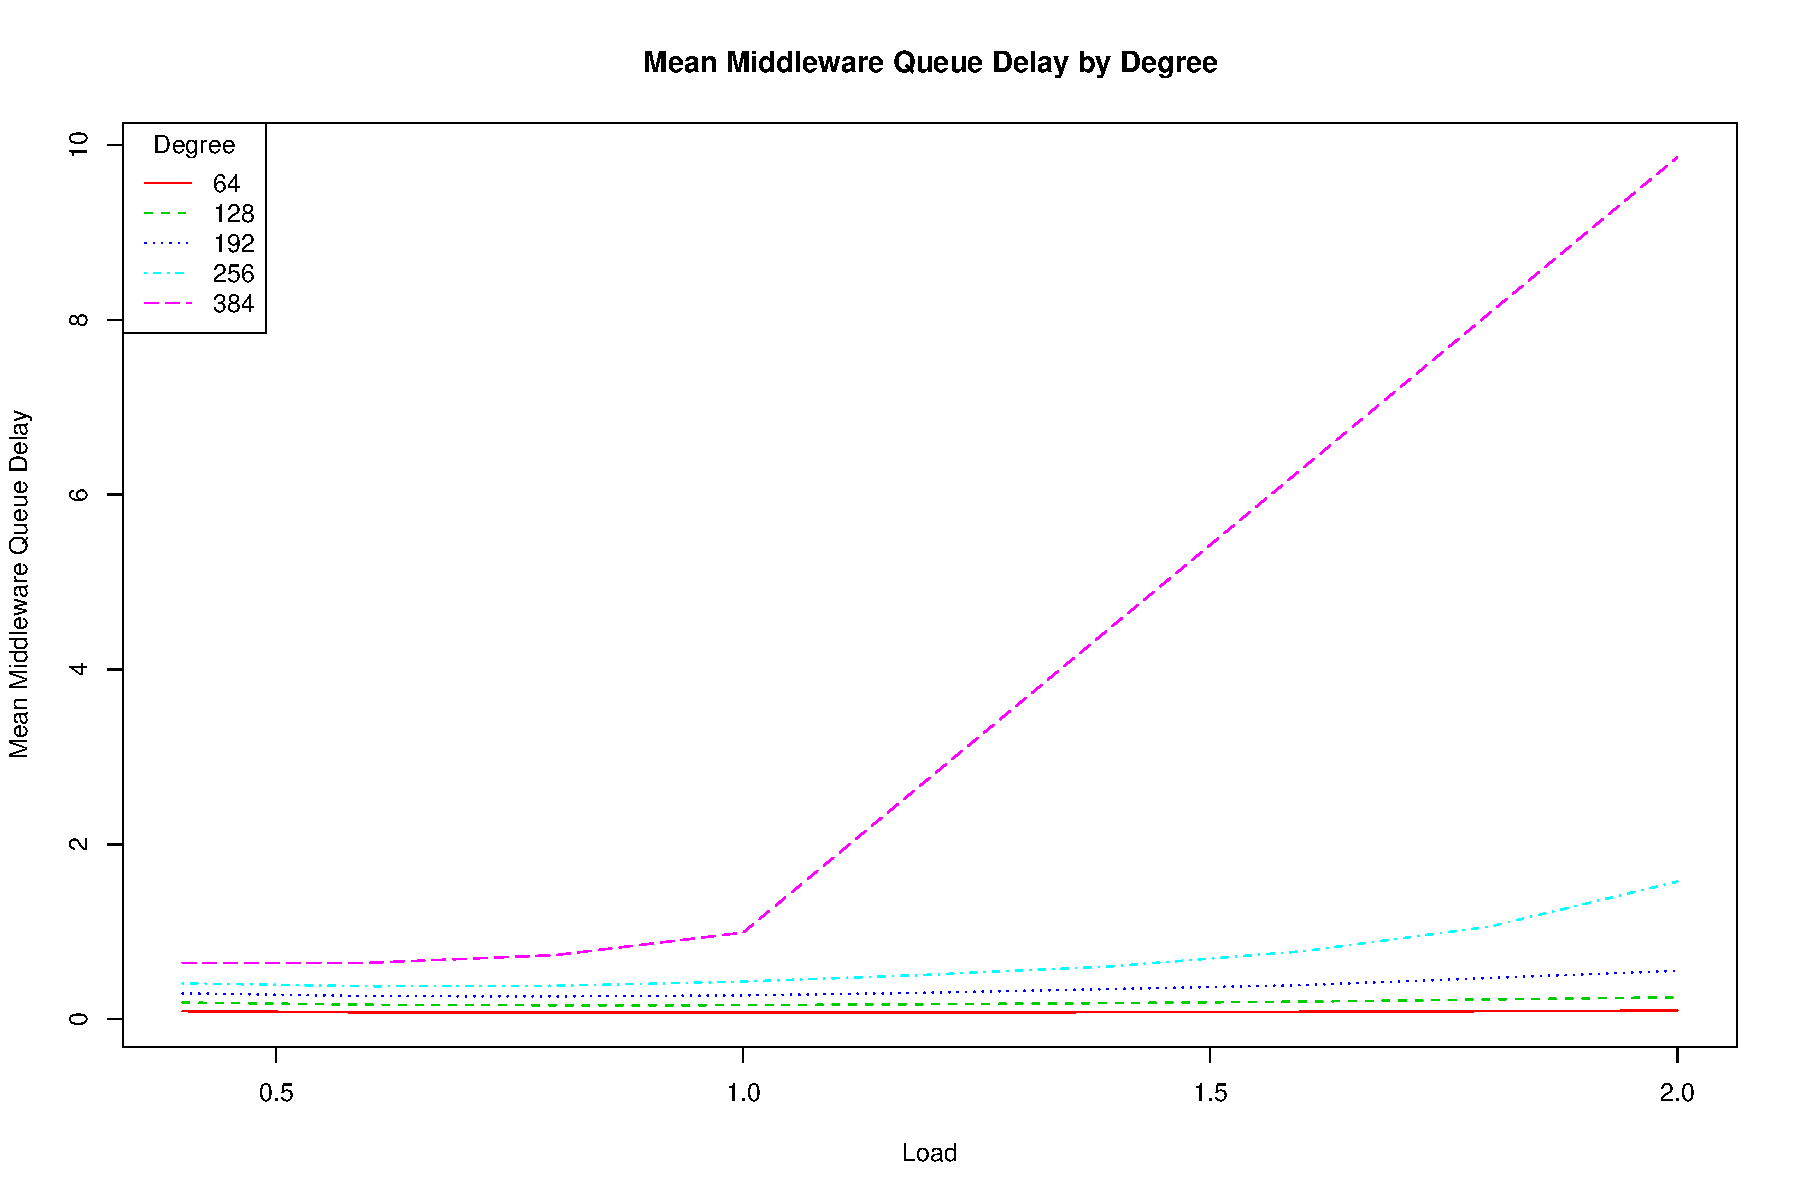
\includegraphics[width=12cm]{appendix/queue_delay_mean}}
  \label{FIG:APX:QDELAY}
  \caption{The mean delay time for messages introduced by having to queue to be
  served. This is a key metric, as even a few seconds delay in being served can
  results offer cancellation and reduce utility and performance, Like in figure
  \ref{FIG:APX:QSIZE}, there is a significant increase for a degree of 384.}
\end{figure}

\begin{figure}[h] 
  \centering
  \fbox{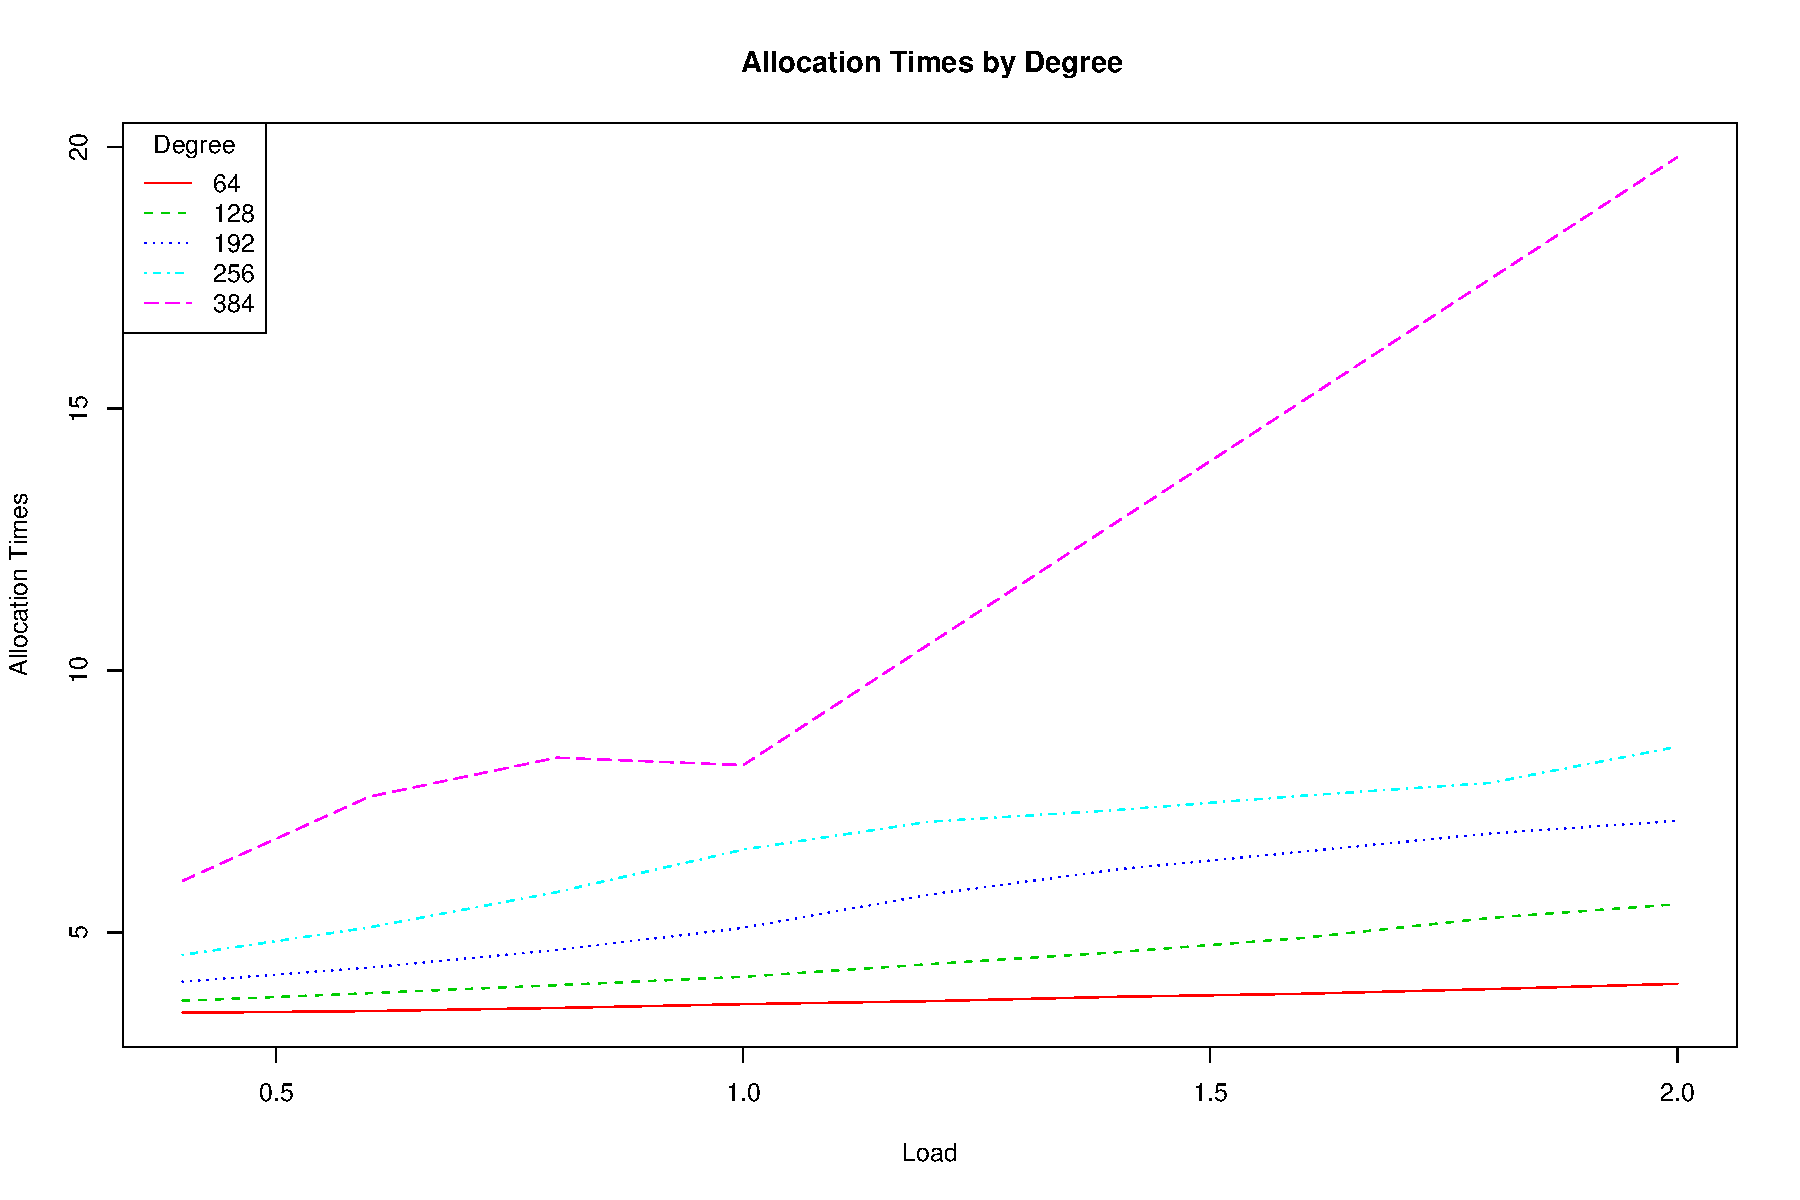
\includegraphics[width=12cm]{appendix/allocation_time_mean}}
  \label{FIG:APX:ALLOCTIME}
  \caption{The mean allocation time by degree. Again, a degree of 256 scales
  less than other values.}
\end{figure}



